\documentclass[11pt,letterpaper]{article}
\usepackage[lmargin=1in,rmargin=1in,tmargin=1in,bmargin=1in]{geometry}
\usepackage{../style/homework}
\usepackage{../style/commands}
\setbool{quotetype}{false} % True: Side; False: Under
\setbool{hideans}{true} % Student: True; Instructor: False

% -------------------
% Content
% -------------------
\begin{document}

\homework{8: Due 03/06}{Laura, clear out the rest of my day! I have to push a boulder up a hill and then have it roll over me time and time again with no regard for my well-being.}{Princess Carolyn, BoJack Horseman}

% Problem 1
\problem{10} Kelsey is gambling at a casino. She is playing a game where you roll two die. If you roll two 6's, you win \$100. If you the dice and the numbers on both die are four or greater (but not two 6's), you win \$10. If the numbers on both die are less than 3, you lose \$8. Otherwise, you win nothing. You must pay \$5 as a `buy-in' each round to play. Find the amount that you win/lose `on average.' Should one play this game?



\newpage



% Problem 2
\problem{10} Find the least square regression line for the points: $(1, 3), (3, 5), (1, 2), (2, 2)$. Show all your work. 



\newpage



% Problem 3
\problem{10} Given the following information below, find the least square regression line. Show all your work. 
	\[
	\begin{aligned}
	n&= 200 \\
	\overline{x}&= 4.42726, \quad \sigma_x^2&= 10.6639 \\
	\overline{y}&= 46.5248, \quad \sigma_y^2&= 1053.77 \\
	R&= 0.962639
	\end{aligned}
	\]



\newpage



% Problem 4
\problem{10} Match each regression coefficient to its corresponding graph. 
	\begin{figure}[!ht]
	\centering
	\begin{minipage}{0.45\textwidth}
	   \centering
	   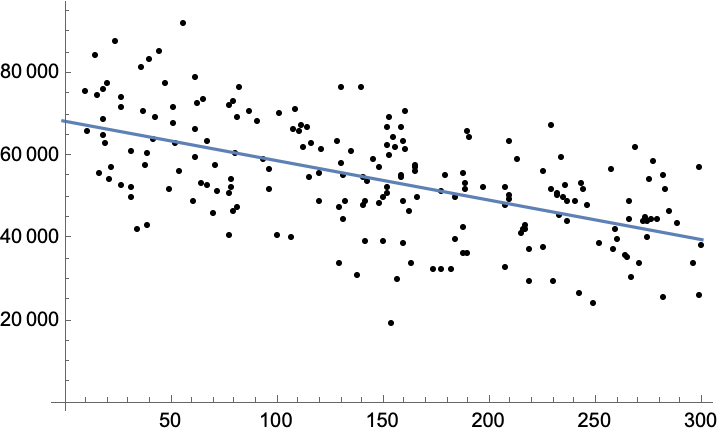
\includegraphics[width=0.9\textwidth]{reg1.png}
	   \caption*{(a)}
	\end{minipage}\hfill
	\begin{minipage}{0.45\textwidth}
	   \centering
	   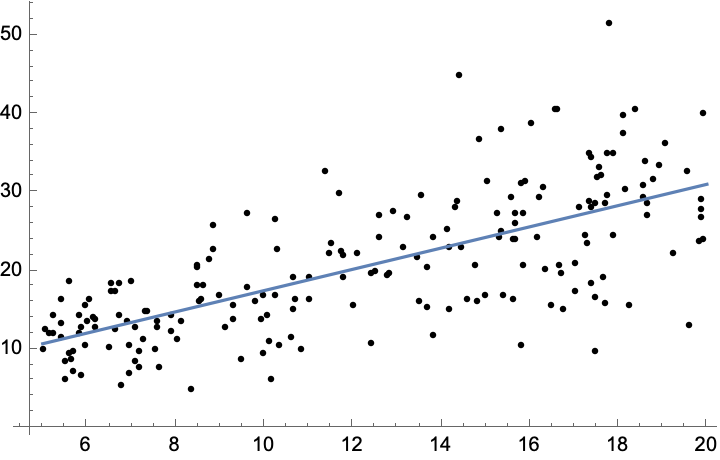
\includegraphics[width=0.9\textwidth]{reg2.png}
	   \caption*{(b)}
	\end{minipage}
	\begin{minipage}{0.45\textwidth}
	   \centering
	   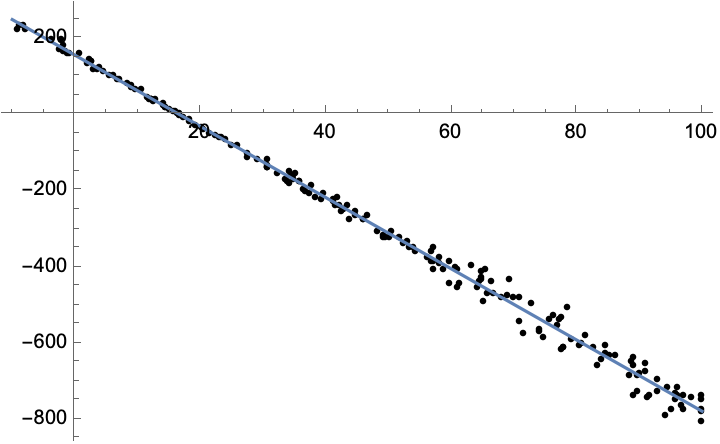
\includegraphics[width=0.9\textwidth]{reg3.png}
	   \caption*{(c)}
	\end{minipage}
	\begin{minipage}{0.45\textwidth}
	   \centering
	   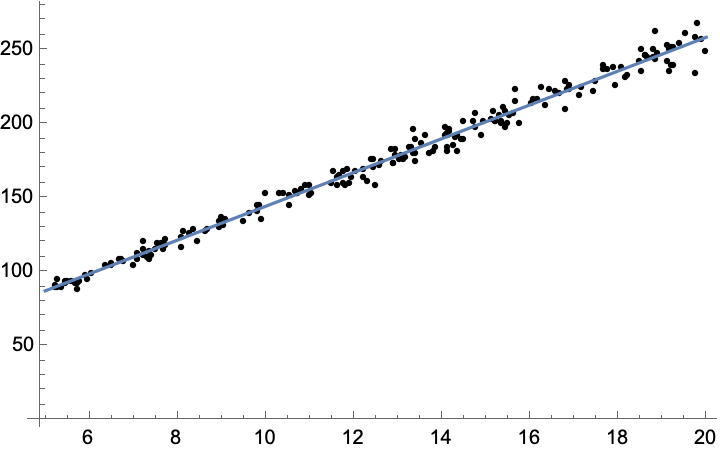
\includegraphics[width=0.9\textwidth]{reg4.png}
	   \caption*{(d)}
	\end{minipage}
	\end{figure}

\begin{enumerate}[(i)]
\item \usol{0.5cm}{}: $R= 0.836288$
\item \usol{0.5cm}{}: $R= -0.998836$
\item \usol{0.5cm}{}: $R= 0.997066$
\item\usol{0.5cm}{}: $R= -0.759531$
\end{enumerate} 


\end{document}